\begin{frame}{Interne datoteke}
	\begin{itemize}
		\item{Git unutar .git direktorija svakog repozitorija sprema datoteke koje sadrže informacije o repozitoriju}
		\item{Neke od tih informacija su popis grana, promjene spremljene u index, konfiguracija, lokacija HEAD-a i sl.}
		\item{Git svim commitovima i podacima pridodaje jedinstvene ključeve (hasheve) koji se koriste za identificiranje i pristup tim podacima i koriste se u internim gitovim datotekama}
	\end{itemize}
\end{frame}
\begin{frame}{Datoteka config}
	\begin{itemize}
		\item{Datoteka config unutar .git direktorija sadrži osnovne podatke o repozitoriju kao što je popis svih povezanih udaljenih repozitorija, poveznicu na master granu zadanog default repozitorija i interne opcije kao što je osjetljivost na velika i mala slova}
		\item{Primjer config datoteke:}
	\end{itemize}
	\begin{center}
		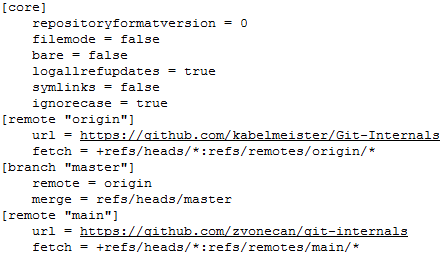
\includegraphics[width=0.66\linewidth]{img/config.png}
	\end{center}
\end{frame}